\subsubsection{\idx{Питагора}}

\zadatak Одреди $x$ са слике.
$$
\slika{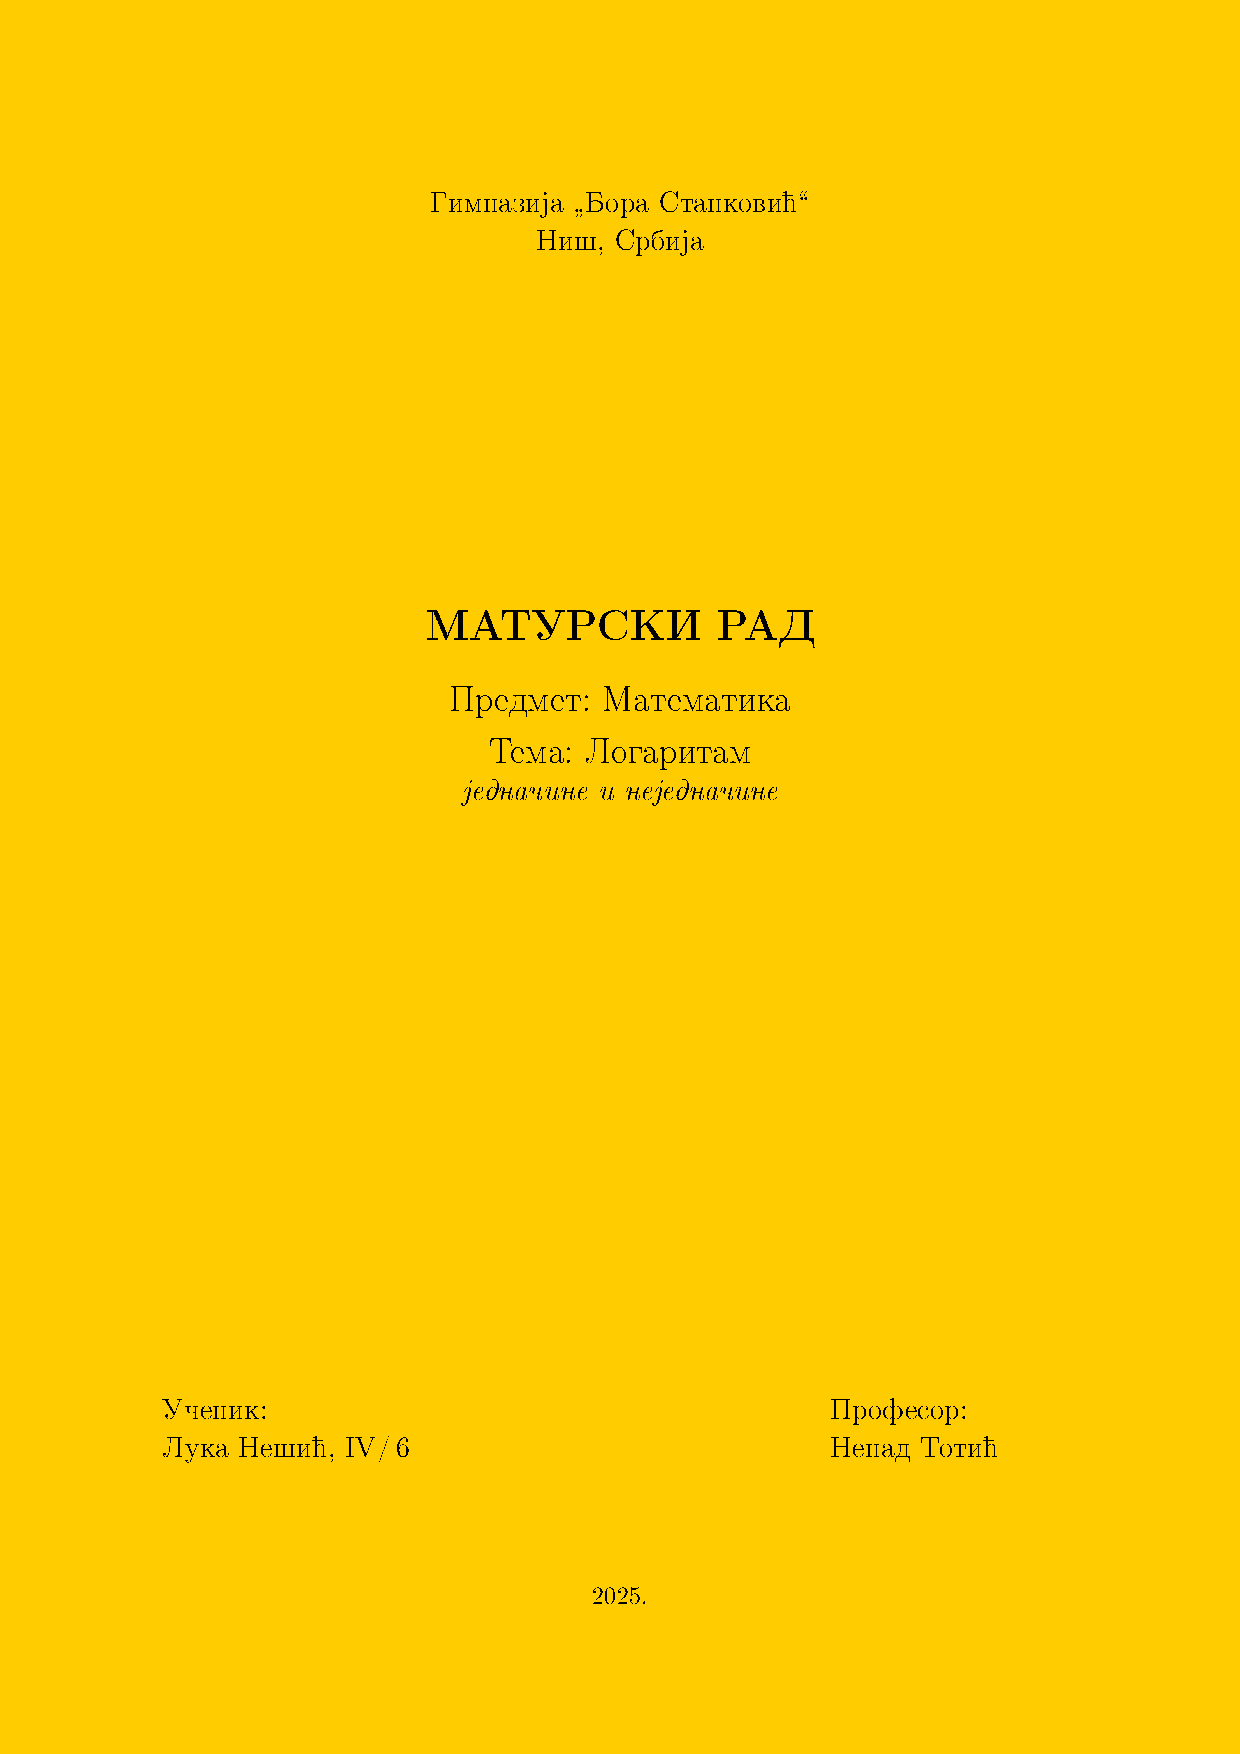
\includegraphics[]{log.5}}{Правоугли троугао\index{троугао $(\triangle)$}\index{правоугли троугао} $\triangle ABC$.}
$$
(Задатак са {Tik-Toka\index{TikTok@Tik-Tok}}.)

\resenje Нађимо најпре решење општег случаја
$$
a=\ln(px),\quad b=\ln(qx),\quad c=\ln(rx).
$$
Због лакшег писања, извршимо смену
$$t=\ln x,\quad u=\ln p,\quad v=\ln q,\quad w=\ln r,$$
одакле је
$$a=t+u,\quad b=t+v,\quad c=t+w.$$
Из {\sl Питагорине теореме\/}\index{Питагорина теорема} 
$a^2 + b^2 = c^2$, следи да је
\begin{align*}
(t+u)^2 + (t+v)^2 &=(t+w)^2\\
t^2 +2tu + u^2 + t^2 + 2tv + v^2 &= t^2 + 2tw + w^2
\end{align*}
где, након сређивања, добијамо квадратну једначину\queq
$$
t^2 + 2(u+v-w)t + (u^2 + v^2 - w^2)=0,
$$
чија су решења\index{антилогаритам}\index{апсолутна вредност $\vert x\vert$}%
\begin{align*}\noalign{\vskip-6pt}
t_{1,2} &=
w-u-v \pm \sqrt{2(w-u)(w-v)},
\intertext{али нас занима само позитивно. Када вратимо смену добијамо}
\ln x &=
\ln\left(\frac{r}{p q}\right) + \sqrt{2\ln\left(\frac rp\right) \ln\left(\frac rq\right)},
\intertext{где је, после антилогаритмовања}
x &= \frac{r}{p q}\cdot\e^{\sqrt{2\ln(r/p)\ln(r/q)}}.
\intertext{Због логаритама испод корена видимо да мора бити $p,q,r>0$ или $p,q,r<0$, и
$|p|,|q|<|r|$, где ће $x$ имати исти знак као $p$, $q$ и $r$.}
\intertext{\indent Када заменимо вредности са слике, 
$p=1$, $q=2$ и $r=3$, добијамо да је}
x &= \ram{\frac32\, \e^{\sqrt{2\ln(3)\ln(3/2)}}}
\approx 3\.85488,
\end{align*}
а странице троугла су приближно
$$
a\approx 1\.34934, \quad b\approx 2\.04249, \quad c\approx 2\.44795.
$$
(На слици је $1=\hbox{`$\vcenter{\hbox{\rule{3truecm}{0.4truept}}}$'}$.)
